% Промежуточный научно-технический отчёт по этапу 1
% Грант ФСИ «Старт-1». Оформление по ГОСТ 7.32 (класс G7-32).
% Титульный лист, список исполнителей и реферат формируются в системе
% «Фонд-М» и в данный документ не включаются (см. рекомендации ФСИ).
\documentclass{G7-32}
% Преамбула отчёта (ГОСТ 7.32).
% Класс G7-32 уже загружает: fontspec, polyglossia (русский/английский),
% amsmath, caption (настройки ГОСТ), geometry (поля ГОСТ), titlesec, tikz,
% multirow, etoolbox. Повторно их не подключаем.

% Моноширинный шрифт (fontspec загружается классом). Liberation Mono входит в
% образ сборки (пакет fonts-liberation) и содержит кириллицу.
\setmonofont{Liberation Mono}

% ГОСТ 7.0.11 требует правое поле 15 мм (класс по умолчанию ставит 10 мм).
\geometry{right=15mm}

% Более мягкая вёрстка абзацев: разрешаем растяжение межсловных интервалов,
% чтобы длинные идентификаторы кода (\texttt) переносились на новую строку,
% а не выходили за правое поле.
\sloppy
\setlength{\emergencystretch}{3em}

% Математика
\usepackage{amsfonts}
\usepackage{amssymb}

% Графика
\usepackage{graphicx}
\usepackage{float}

% Схемы (архитектура вычислительного слоя, конвейер симуляции)
\usepackage{tikz}
\usetikzlibrary{arrows.meta, positioning}
% Кинематические схемы (глава о генерации кинематики из STEP)
\usepackage{kinematikz}

% Таблицы
\usepackage{booktabs}
\usepackage{array}
\usepackage{longtable}

% Цвет
\usepackage{xcolor}

% Листинги исходного кода
\usepackage{listings}
\definecolor{lstkw}{rgb}{0.0,0.0,0.5}
\definecolor{lstcomment}{rgb}{0.30,0.45,0.30}
\definecolor{lststring}{rgb}{0.55,0.10,0.10}
\lstset{
  basicstyle=\footnotesize\ttfamily,
  keywordstyle=\color{lstkw}\bfseries,
  commentstyle=\color{lstcomment}\itshape,
  stringstyle=\color{lststring},
  breaklines=true,
  frame=single,
  numbers=left,
  numberstyle=\tiny,
  showstringspaces=false,
  tabsize=2,
  captionpos=b,
  columns=fullflexible,
  keepspaces=true,
}
% Подпись листингов на русском
\renewcommand{\lstlistingname}{Листинг}

% --- Псевдокод ---------------------------------------------------------------
% Алгоритмы оформляются псевдокодом в обрамлённом блоке; нумерация общая с
% листингами. Использование:
%   \begin{pseudocode}{<подпись>}{<метка>}
%     строки псевдокода, отступ уровня n --- \pind{n}, перенос строки --- \\
%   \end{pseudocode}
\newcommand{\pind}[1]{\hspace*{#1\dimexpr1.6em\relax}}
\newsavebox{\pseudobox}
\newenvironment{pseudocode}[2]{%
  \par\medskip\noindent
  \begin{minipage}{\linewidth}%
  \def\pseudocaption{#1}\def\pseudolabel{#2}%
  \setlength{\fboxsep}{8pt}%
  \begin{lrbox}{\pseudobox}%
  \begin{minipage}{\dimexpr\linewidth-2\fboxsep-2\fboxrule\relax}%
  \small\setlength{\parindent}{0pt}\raggedright
}{%
  \end{minipage}\end{lrbox}%
  \noindent\fbox{\usebox{\pseudobox}}\par\smallskip
  \captionof{lstlisting}{\pseudocaption}\label{\pseudolabel}%
  \end{minipage}\par\medskip
}

% Гиперссылки (подключать последними)
\usepackage{hyperref}
\hypersetup{
  colorlinks=true,
  linkcolor=black,
  citecolor=black,
  urlcolor=blue,
  pdftitle={Промежуточный научно-технический отчёт по этапу 1},
  pdfauthor={farfield},
}

% --- Заглушка под скриншот -------------------------------------------------
% Использование:
%   \screenshot{<доля \textwidth>}{<подпись рисунка>}{<что заснять>}{<метка>}
% Рисует обрамлённую область с пояснением; нумеруется как обычный рисунок и
% попадает в список иллюстраций. Когда изображение готово, заглушку заменяют
% на \includegraphics из каталога figures/.
\newcommand{\screenshot}[4]{%
  \begin{figure}[ht]\centering
    \setlength{\fboxsep}{0pt}%
    \fbox{\begin{minipage}[c][0.40\textwidth][c]{#1\textwidth}%
      \centering
      \itshape\small[\,ЗАГЛУШКА ДЛЯ СКРИНШОТА\,]\par\medskip
      \normalfont\small #3\par\medskip
      \footnotesize\ttfamily figures/#4.png
    \end{minipage}}%
    \caption{#2}\label{fig:#4}
  \end{figure}%
}


\begin{document}

\frontmatter % ненумерованная часть

\tableofcontents

\chapter*{ВВЕДЕНИЕ}
\addcontentsline{toc}{chapter}{ВВЕДЕНИЕ}

Настоящий документ представляет собой промежуточный научно-технический отчёт о
выполнении первого этапа научно-исследовательской и опытно-конструкторской
работы (НИОКР) по теме <<Разработка и тестирование прототипа программного
комплекса для моделирования и симуляции роботов с использованием графических
ускорителей>>, выполняемой при поддержке Фонда содействия инновациям по
программе <<Старт-1>>. Отчёт оформлен в соответствии с требованиями
ГОСТ~7.32~\cite{gost732}.

\textbf{Актуальность работы.}
Робототехника является одной из наиболее динамично развивающихся областей
современной техники. Проектирование, верификация и тестирование
робототехнических систем требуют значительных временны\'{х} и финансовых затрат
при работе с физическим оборудованием. Программные комплексы моделирования и
симуляции позволяют перенести значительную часть этих работ в виртуальную среду,
сокращая цикл разработки, снижая риски повреждения дорогостоящего оборудования и
обеспечивая воспроизводимость экспериментов. Современные сценарии применения ---
обучение с подкреплением, построение цифровых двойников, отработка алгоритмов
управления --- предъявляют всё более высокие требования к производительности
симуляции, что делает применение графических ускорителей (GPU) для расчёта
физической динамики не только желательным, но и необходимым.

В условиях ограничений на использование зарубежного программного обеспечения
актуальность создания отечественного программного комплекса робототехнической
симуляции существенно возрастает. Разрабатываемый комплекс ориентирован на
импортонезависимую инженерную разработку и объединяет средства загрузки и
визуализации моделей роботов и сцен, автоматического построения кинематических
схем, физической симуляции с GPU-ускорением и графический интерфейс
пользователя.

\textbf{Цель этапа.}
Целью первого этапа является разработка и тестирование отдельных подсистем
прототипа программного комплекса: модулей загрузки и отрисовки моделей роботов и
сцен, алгоритма построения кинематической схемы, алгоритмов симуляции на
центральном (CPU) и графическом (GPU) процессорах, а также базового графического
интерфейса пользователя, с проведением предварительного тестирования на
искусственных данных и сбором эталонных показателей производительности.

\textbf{Задачи этапа} соответствуют работам календарного плана:
\begin{enumerate}
  \item разработка и реализация алгоритма загрузки и отрисовки моделей роботов в
        формате URDF;
  \item реализация модуля загрузки моделей сцен и объектов окружения в форматах
        SDF и STL;
  \item разработка и программная реализация алгоритма генерации кинематической
        схемы на основе формата STEP;
  \item разработка и реализация алгоритма симуляции, не использующего
        графический процессор;
  \item разработка и тестирование базового графического интерфейса пользователя;
  \item предварительное тестирование прототипа программного комплекса на
        искусственных данных и сбор эталонных показателей;
  \item разработка и программная реализация алгоритма численного интегрирования
        дифференциальных уравнений с помощью GPU.
\end{enumerate}

\textbf{Место этапа в выполнении НИОКР в целом.}
Первый этап закладывает функциональный фундамент программного комплекса. На нём
создаются независимо тестируемые подсистемы (загрузка моделей, построение
кинематики, физическое ядро, интерфейс) и формируется набор эталонных
показателей, относительно которых на последующих этапах будет оцениваться
прирост производительности и точности при масштабировании GPU-ускорения и
интеграции подсистем в единый прикладной комплекс.

\textbf{Структура отчёта.}
Основная часть отчёта построена в соответствии с календарным планом. Раздел~1
обосновывает выбор направления исследований и общую методику. Разделы~2--8
описывают результаты по каждой из работ этапа. Раздел~9 содержит обобщение и
оценку полученных результатов. В заключении приведены краткие выводы и оценка
полноты решения поставленных задач.

\textbf{Программные результаты этапа} размещены в следующих репозиториях:
\begin{itemize}
  \item \texttt{modeuler} --- загрузка и отрисовка моделей в формате URDF,
        загрузка и отрисовка сцен в форматах SDF и STL;
  \item \texttt{kinechain} --- алгоритм генерации кинематической схемы из файлов
        в формате STEP;
  \item \texttt{modeuler-win} --- базовый графический интерфейс пользователя;
  \item \texttt{dyphur} --- алгоритм симуляции и решатель (солвер)
        дифференциальных уравнений с помощью GPU.
\end{itemize}


\mainmatter % включает нумерацию разделов

\chapter{ВЫБОР НАПРАВЛЕНИЯ ИССЛЕДОВАНИЙ И ОБЩАЯ МЕТОДИКА}
\label{cha:method}

\section{Обоснование направления исследований}

Разрабатываемый программный комплекс предназначен для моделирования и симуляции
робототехнических систем. Анализ предметной области и существующих решений
позволил выделить функциональные блоки, совокупность которых обеспечивает полный
цикл подготовки и проведения виртуального эксперимента:

\begin{enumerate}
  \item \textbf{Импорт и визуализация моделей.} Модели роботов в робототехнике
        традиционно описываются форматом URDF (Unified Robot Description Format),
        а сцены и объекты окружения --- форматами SDF (Simulation Description
        Format) и STL (стереолитография). Комплекс должен загружать эти форматы и
        отображать их в трёхмерной сцене в реальном времени.
  \item \textbf{Автоматическое построение кинематики.} Конструкторская
        документация на изделия чаще всего поставляется в нейтральном формате
        STEP (ISO~10303), который описывает геометрию сборки, но не содержит
        сведений о подвижных соединениях. Требуется алгоритм, восстанавливающий
        кинематическую схему (дерево звеньев и суставов) из геометрии сборки.
  \item \textbf{Физическая симуляция.} Ядро комплекса --- решатель динамики
        твёрдых тел с обнаружением столкновений и обработкой контактных
        ограничений. Для оптимизации трудозатрат принято решение в пользу
        единой кросс-платформенной реализации: один и тот же код исполняется
        как на центральном процессоре (CPU), так и на графических ускорителях
        (GPU) разных производителей, что исключает дублирование
        алгоритмической логики и расхождение версий.
  \item \textbf{Графический интерфейс пользователя.} Прикладная оболочка,
        объединяющая перечисленные подсистемы в единый рабочий процесс.
\end{enumerate}

\section{Сравнительный обзор существующих решений}

Задача физического моделирования твёрдых тел в робототехнике изучается с
1990-х~годов; основополагающие работы Д.~Барафа и А.~Уиткина~\cite{baraff1997}
заложили теоретическую базу контактной динамики. На сегодняшний день существует
ряд широко используемых систем~\cite{todorov2012mujoco,coumans2021bullet,nvidia_physx,smith2005ode}
(таблица~\ref{tab:engines}).

\begin{table}[ht]
  \centering
  \caption{Сравнение систем робототехнической симуляции}
  \label{tab:engines}
  \small
  \begin{tabular}{p{0.20\textwidth} p{0.30\textwidth} p{0.18\textwidth} p{0.18\textwidth}}
    \toprule
    Система & Физическое ядро & GPU-ускорение & Лицензия \\
    \midrule
    Gazebo / Ignition & ODE, Bullet, DART & Нет & Apache 2.0 \\
    MuJoCo            & Собственное (мягкие контакты) & Частично (MJX) & Apache 2.0 \\
    NVIDIA Isaac Sim  & PhysX 5 & Да & Проприетарная \\
    CoppeliaSim       & ODE, Bullet, Vortex, Newton & Нет & Проприетарная/\allowbreak GPL \\
    PyBullet          & Bullet & Нет & Zlib \\
    \bottomrule
  \end{tabular}
\end{table}

Перечисленные решения, как правило, не объединяют в одном продукте удобную среду
визуального моделирования, высокоточную симуляцию с массовым GPU-ускорением и
средства автоматической подготовки моделей из конструкторской документации.
Кроме того, ряд систем распространяется на условиях лицензий, ограничивающих
применение в государственном и коммерческом секторах. Это подтверждает
целесообразность разработки собственного комплекса.

\section{Методы решения задач и архитектура комплекса}

Прототип построен по модульному принципу. Подсистемы разделены по
ответственности и взаимодействуют через явно определённые программные
интерфейсы, что позволяет разрабатывать и тестировать их независимо
(рисунок~\ref{fig:arch}).

\begin{itemize}
  \item \texttt{modeuler} --- модуль загрузки и визуализации (C++); отрисовка
        выполняется средствами VulkanSceneGraph~\cite{vsg} поверх графического API Vulkan~\cite{vulkan};
  \item \texttt{kinechain} --- инструмент построения кинематической схемы из STEP
        (Python, геометрическое ядро OpenCASCADE~\cite{opencascade});
  \item \texttt{dyphur} --- физическое ядро (C++20) с переносимым вычислительным
        слоем поверх SYCL/AdaptiveCpp: единый исходный код компилируется для
        бэкендов CUDA (NVIDIA), HIP (AMD ROCm) и OpenMP (CPU);
  \item \texttt{modeuler-win} --- графический интерфейс пользователя (C\#, WPF).
\end{itemize}

\screenshot{0.7}{Архитектура прототипа программного комплекса}{Снимок экрана:
схема взаимодействия подсистем (modeuler, kinechain, dyphur, modeuler-win) ---
блок-схема компонентов и потоков данных между ними.}{arch}

\section{Общая методика проведения работ}

Разработка велась по итеративной методике с обязательным автоматизированным
тестированием. Для каждого модуля:
\begin{enumerate}
  \item формулировались функциональные требования и критерии приёмки;
  \item реализовывался алгоритм с покрытием модульными тестами;
  \item проводилось предварительное тестирование на искусственных
        (синтетических) данных, для которых известен ожидаемый результат;
  \item фиксировались эталонные показатели (корректность, детерминизм,
        производительность), используемые как опорные значения на последующих
        этапах.
\end{enumerate}

Воспроизводимость результатов обеспечивается контейнеризацией среды сборки и
фиксацией версий зависимостей. Особое внимание уделено \emph{детерминизму}
физического ядра: при фиксированных сборке и аппаратной платформе результаты
симуляции должны быть побитово воспроизводимыми, что является необходимым
условием для верификации алгоритмов управления и отладки.

\chapter{ЗАГРУЗКА И ОТРИСОВКА МОДЕЛЕЙ РОБОТОВ В ФОРМАТЕ URDF}
\label{cha:urdf}

\section{Постановка задачи}

URDF (Unified Robot Description Format)~\cite{urdf} --- основанный на XML формат
описания кинематической структуры робота: набор твёрдых звеньев (\texttt{link}),
соединённых суставами (\texttt{joint}). Каждое звено содержит визуальную
(\texttt{visual}), столкновительную (\texttt{collision}) и инерционную
(\texttt{inertial}) геометрию; сустав задаёт тип сочленения (вращательное,
призматическое, фиксированное и др.), оси, пределы и взаимное расположение
родительского и дочернего звеньев. Задача состоит в загрузке URDF-модели,
построении дерева звеньев и его визуализации в трёхмерной сцене с возможностью
интерактивного управления.

Работа выполнена в репозитории \texttt{modeuler}, модуль \texttt{scene}.

\section{Алгоритм загрузки}

Разбор URDF выполняется в два прохода. На первом проходе извлекаются все звенья и
суставы с их атрибутами и геометрией. На втором --- по родительско-дочерним
связям суставов строится дерево звеньев, вычисляются относительные
преобразования и определяется корневое звено (звено, не являющееся дочерним ни
для одного сустава). Преобразования заданы в виде однородных матриц $4\times4$;
положение звена в мировой системе координат получается перемножением
преобразований вдоль пути от корня.

\begin{lstlisting}[language=C++,caption={Разбор URDF и построение дерева звеньев (схематично)},label=lst:urdf]
UrdfModel load_urdf(const std::filesystem::path& path) {
    auto xml = parse_xml(path);                    // pugixml
    UrdfModel model;
    for (auto& link : xml.select("robot/link"))
        model.links.emplace(link.attr("name"), parse_link(link));
    for (auto& joint : xml.select("robot/joint")) {
        Joint j = parse_joint(joint);              // type, axis, origin, limits
        model.links[j.child].parent_joint = j.name;
        model.joints.emplace(j.name, std::move(j));
    }
    model.root = find_root_link(model);            // звено без родительского сустава
    compute_world_transforms(model, model.root);   // обход дерева в глубину
    return model;
}
\end{lstlisting}

Каждому визуальному элементу звена сопоставляется примитив (бокс, цилиндр, сфера)
или загружаемая полигональная сетка (mesh). Загрузка сеток и материалов
выполняется средствами библиотеки vsgXchange, что обеспечивает поддержку
распространённых форматов геометрии. Описание звеньев и суставов хранится в
структурах \texttt{Link} и \texttt{Joint} (заголовки \texttt{models/link.hpp},
\texttt{models/joint.hpp}).

\section{Отрисовка}

Визуализация построена на VulkanSceneGraph (VSG)~\cite{vsg} --- современной
библиотеке графа сцены поверх графического API Vulkan~\cite{vulkan}. Для каждого звена создаётся узел графа
сцены с матрицей преобразования; визуальная геометрия звена присоединяется как
дочерний узел. Это позволяет при изменении обобщённых координат сустава
обновлять лишь соответствующую матрицу, не пересобирая граф сцены.

Подсистема визуализации включает (модуль \texttt{scene}):
\begin{itemize}
  \item управление камерой и навигацией (\texttt{utils/camera.hpp},
        \texttt{controllers/arcball\_controller}) --- орбитальное вращение,
        панорамирование, масштабирование;
  \item выбор объектов сцены (\texttt{controllers/picking\_controller}) ---
        определение звена под курсором методом трассировки луча;
  \item интерактивное вращение суставов
        (\texttt{controllers/\allowbreak joint\_rotation\_controller}) --- изменение
        обобщённой координаты вращательного сустава перетаскиванием;
  \item вспомогательные элементы (\texttt{utils/arrow\_gizmo}) --- визуализация
        осей и манипуляторов.
\end{itemize}

\screenshot{0.85}{Загруженная URDF-модель робота в трёхмерной сцене}{Снимок
экрана: окно просмотра \texttt{modeuler} с загруженной моделью манипулятора в
формате URDF; видны звенья, оси суставов и элементы управления камерой.}{urdf-view}

\section{Результаты}

Реализованы загрузка URDF-моделей, построение дерева звеньев с вычислением
мировых преобразований и интерактивная визуализация в реальном времени.
Поддержаны основные типы суставов и базовые визуальные примитивы, а также
загрузка полигональных сеток. Корректность построения дерева и преобразований
проверена на тестовых моделях с известной кинематикой; результат соответствует
ожидаемому расположению звеньев.

\chapter{ЗАГРУЗКА МОДЕЛЕЙ СЦЕН И ОБЪЕКТОВ ОКРУЖЕНИЯ В ФОРМАТАХ SDF И STL}
\label{cha:sdf}

\section{Постановка задачи}

Помимо моделей роботов, для проведения виртуального эксперимента необходимо
описание рабочей сцены: статического окружения, препятствий, объектов
манипулирования. Для этого применяются форматы:
\begin{itemize}
  \item \textbf{SDF} (Simulation Description Format)~\cite{sdformat} ---
        основанный на XML формат описания сцены (мир, модели, звенья, суставы, источники света, физические
        свойства); фактический стандарт в экосистеме Gazebo;
  \item \textbf{STL} (STereoLithography) --- формат хранения полигональной
        (треугольной) сетки, широко используемый для представления геометрии
        деталей и препятствий.
\end{itemize}

Задача --- реализовать загрузку сцен SDF и геометрии STL и их отображение в той
же трёхмерной сцене, что и модели роботов. Работа выполнена в репозитории
\texttt{modeuler} (модуль \texttt{scene}, компоненты \texttt{utils/scene\_loader},
\texttt{utils/model\_loader}, \texttt{utils/scene\_manager}).

\section{Загрузка сцен SDF}

Разбор SDF выполняется аналогично URDF: дерево XML обходится с извлечением
вложенных моделей, звеньев и их геометрии; для каждой модели строится локальная
система координат, а модели размещаются в мировой системе согласно заданным
позам (\texttt{pose}). Поскольку SDF и URDF имеют близкую объектную модель
(звенья, суставы, геометрия, позы), в \texttt{modeuler} они приводятся к единому
внутреннему представлению сцены (\texttt{scene.hpp}), что позволяет переиспользовать
конвейер отрисовки и подсистему управления камерой.

\section{Загрузка геометрии STL}

Загрузка STL реализована через vsgXchange: бинарные и текстовые STL-файлы
преобразуются в узлы графа сцены с буферами вершин и нормалей. Для отсутствующих
нормалей выполняется их восстановление по граням. Загруженная сетка
присоединяется к узлу соответствующего объекта сцены и далее обрабатывается
конвейером отрисовки наравне с прочей геометрией.

\begin{figure}[ht]
  \centering
  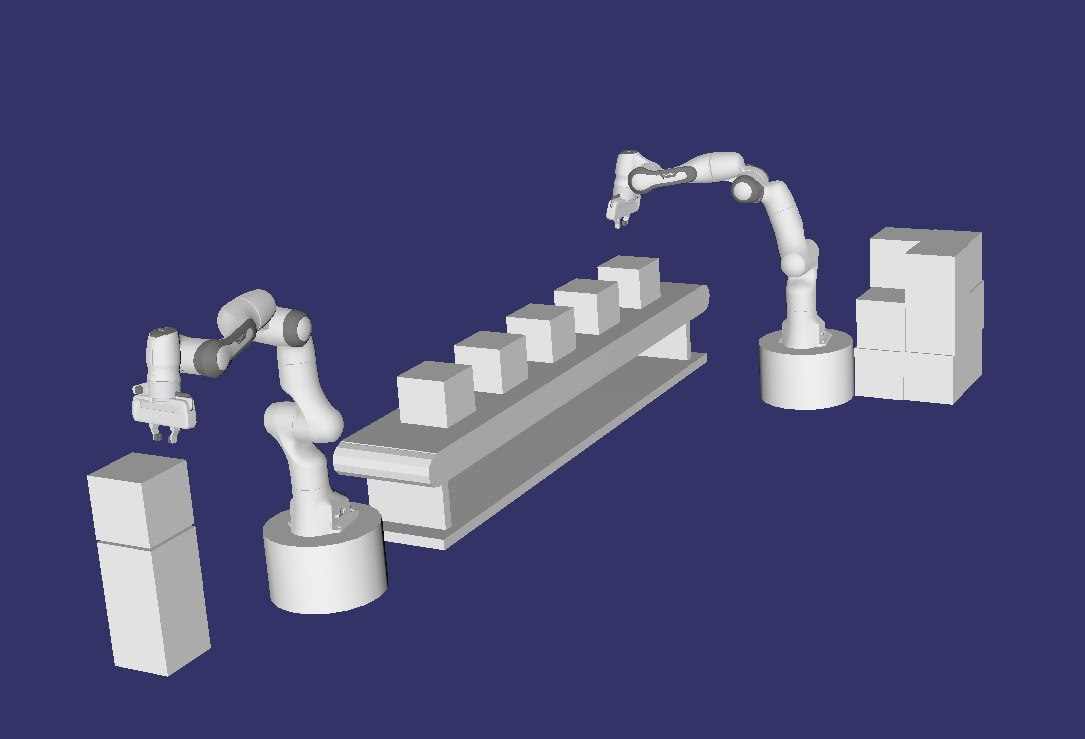
\includegraphics[width=0.9\textwidth]{figures/modeuler-scene.jpg}
  \caption{Загруженная рабочая сцена: конвейерная линия с двумя манипуляторами
    и объектами окружения}
  \label{fig:sdf-scene}
\end{figure}

Пример загруженной сцены показан на рисунке~\ref{fig:sdf-scene}: рабочая ячейка
с конвейерной линией, двумя манипуляторами и объектами манипулирования;
статическое окружение и полигональная геометрия объектов импортированы из
описания сцены и отображаются совместно с моделями роботов.

\section{Результаты}

Реализованы модуль загрузки сцен в формате SDF и модуль импорта полигональной
геометрии в формате STL. Оба источника приводятся к единому внутреннему
представлению сцены и визуализируются совместно с моделями роботов. Загрузка
проверена на наборе тестовых сцен; объекты размещаются в соответствии с
заданными в SDF позами, геометрия STL отображается без искажений.

\chapter{ГЕНЕРАЦИЯ КИНЕМАТИЧЕСКОЙ СХЕМЫ НА ОСНОВЕ ФОРМАТА STEP}
\label{cha:step}

\section{Постановка задачи}

Конструкторская документация на робототехнические изделия чаще всего
поставляется в нейтральном формате STEP (ISO~10303)~\cite{iso10303}, который
описывает геометрию сборки и иерархию деталей, но \emph{не содержит} сведений о
подвижных соединениях (сопряжениях, mate-связях). Для использования такой
сборки в симуляции необходимо восстановить её кинематическую схему: дерево
звеньев и суставов с их типами и осями, инерционные характеристики звеньев и
описание модели в формате, пригодном для симулятора. Задача решена в
репозитории \texttt{kinechain} (язык Python, геометрическое ядро
OpenCASCADE~\cite{opencascade} через пакет \texttt{cadquery-ocp}); работа по
данному пункту календарного плана завершена.

\section{Конвейер обработки}

Инструмент организован как линейный конвейер, по одному модулю на стадию:

\begin{enumerate}
  \item \textbf{Загрузка STEP} (\texttt{io\_step}): чтение сборки с сохранением
        иерархии и мировых преобразований; на выходе --- плоский список
        именованных деталей, геометрия которых уже приведена к мировой системе
        координат.
  \item \textbf{Извлечение аналитических поверхностей} (\texttt{surfaces}): из
        граничного представления (B-Rep) каждой детали извлекаются плоскости
        (точка, нормаль) и цилиндры (ось, точка на оси, радиус, осевая
        протяжённость).
  \item \textbf{Обнаружение контактов} (\texttt{contact}): широкая фаза по
        перекрытию ограничивающих параллелепипедов (AABB), узкая фаза ---
        проверки геометрической совместности пар поверхностей; на выходе ---
        типизированные \emph{признаки контакта} пары деталей.
  \item \textbf{Классификация суставов} (\texttt{joints}): детерминированные
        правила распознают по признакам контакта вращательный
        (\texttt{revolute}), поступательный (\texttt{prismatic}) или
        фиксированный (\texttt{fixed}) сустав.
  \item \textbf{Построение кинематического дерева} (\texttt{graph}): остовное
        дерево обходом в ширину от корня; не вошедшие в остов суставы
        становятся замыкающими ограничениями циклов.
  \item \textbf{Экспорт} (\texttt{export\_mjcf}, \texttt{export\_sdf}): запись
        модели в MJCF (MuJoCo) или SDF из общего промежуточного представления,
        с выгрузкой полигональных сеток деталей в STL.
\end{enumerate}

Все геометрические допуски (линейный, угловой, по радиусу, минимальные площади
контакта) собраны в одной структуре и выводятся из диагонали ограничивающего
параллелепипеда всей сборки, что делает конвейер \emph{масштабно-инвариантным}:
одни и те же правила работают на сборках от часового до строительного масштаба
без перенастройки.

\section{Обнаружение контактов}

Широкая фаза отбрасывает заведомо не соприкасающиеся пары деталей по перекрытию
AABB (с зазором, равным линейному допуску). Для оставшихся пар узкая фаза
проверяет два вида совместности поверхностей.

\textbf{Соосность цилиндров.} Для цилиндров с осями $\mathbf{a}_1,\mathbf{a}_2$
и точками на осях $\mathbf{p}_1,\mathbf{p}_2$ требуется одновременное
выполнение условий параллельности осей и совпадения прямых:
\begin{equation}
  \lVert \mathbf{a}_1 \times \mathbf{a}_2 \rVert < \varepsilon_{\angle},
  \qquad
  \bigl\lVert (\mathbf{p}_2 - \mathbf{p}_1) \times \mathbf{a}_1 \bigr\rVert
  < \varepsilon_{d},
  \label{eq:coaxial}
\end{equation}
где $\varepsilon_{\angle}$ и $\varepsilon_{d}$ --- угловой и линейный допуски;
дополнительно радиусы должны совпадать в пределах допуска. Для каждой соосной
пары вычисляется \emph{осевое перекрытие} --- длина общего участка вдоль оси,
используемая затем классификатором.

\textbf{Прилегание плоскостей.} Две плоские грани считаются совмещёнными при
параллельности нормалей и расстоянии между плоскостями в пределах допуска;
признак \emph{встречности} нормалей отличает настоящий контакт <<грань к
грани>> от заподлицо расположенных граней. Площадь контакта вычисляется
\emph{точно} (с точностью до триангуляции): триангуляции обеих граней
проецируются на общую плоскость, и суммируется площадь попарных пересечений
треугольников, найденных алгоритмом отсечения выпуклых многоугольников
Сазерленда--Ходжмана. Это корректно даёт нулевую площадь для компланарных, но
не перекрывающихся граней.

\section{Классификация суставов}

Классификация построена на детерминированных правилах, применяемых в порядке
от наиболее ограничивающего типа к наименее: фиксированный $\rightarrow$
поступательный $\rightarrow$ вращательный (листинг~\ref{lst:joint-rules}).
Правила \emph{консервативны}: если ни одно не сработало, пара остаётся
несоединённой и попадает в диагностику, а не <<приваривается>> молча.

\begin{pseudocode}{Алгоритм классификации сустава по признакам контакта}{lst:joint-rules}
\pind0 Вход: соосные пары цилиндров $CC$, совмещённые пары плоскостей $PP$,
       допуски\\
\pind0 $\Pi \leftarrow \{\,p \in PP :$ нормали встречные, площадь контакта
       $\ge S_{\min}\,\}$\\
\pind0 $N \leftarrow$ различные (с точностью до знака) нормали пар из $\Pi$\\
\pind0 \textit{// 1. Фиксированный}\\
\pind0 если $\Pi \neq \varnothing$ и (в $CC$ есть <<болтовая>> пара
       (перекрытие $<$ диаметра)\\
\pind2 или $|N| \ge 2$ и у $N$ нет общего перпендикуляра):\\
\pind1 вернуть \texttt{fixed} с якорем на плоскости наибольшей площади\\
\pind0 \textit{// 2. Поступательный}\\
\pind0 $\mathbf{s} \leftarrow$ общий перпендикуляр ко всем нормалям из $N$
       (существует при $|N| \ge 2$)\\
\pind0 если $\mathbf{s}$ существует и ось каждой пары из $CC$ параллельна
       $\mathbf{s}$:\\
\pind1 вернуть \texttt{prismatic} с осью $\mathbf{s}$\\
\pind0 \textit{// 3. Вращательный}\\
\pind0 если в $CC$ есть пара: перекрытие $\ge$ диаметра и в $\Pi$ нет
       плоскости с нормалью вдоль её оси:\\
\pind1 вернуть \texttt{revolute} с осью этой пары\\
\pind0 иначе вернуть <<нет сустава>> \quad\textit{// пара остаётся
       несоединённой, выводится в диагностику}
\end{pseudocode}

Содержательная основа правил --- анализ степеней свободы, оставляемых
контактами:
\begin{itemize}
  \item \emph{поступательный}: два и более контактов <<грань к грани>> с
        непараллельными нормалями запрещают все вращения и все перемещения,
        кроме одного --- вдоль общего перпендикуляра $\mathbf{s}$ к нормалям
        контактов (направления скольжения); соосный цилиндр при этом не должен
        противоречить $\mathbf{s}$, иначе скольжение разорвало бы контакт;
  \item \emph{фиксированный}: нормали контактов, не имеющие общего
        перпендикуляра, запрещают и последнее перемещение --- пара сварена
        самой геометрией; короткая <<болтовая>> соосная пара (осевое перекрытие
        меньше диаметра --- шпилька или болт, а не подшипниковая посадка) в
        сочетании с прилеганием плоскостей также трактуется как крепёж;
  \item \emph{вращательный}: длинная соосная пара (перекрытие не меньше
        диаметра) без <<заплечика>> --- прилегающей плоскости с нормалью вдоль
        оси, которая исключила бы свободное вращение.
\end{itemize}

Ключевой фрагмент реализации --- вычисление направления скольжения и цепочка
правил --- приведён в листинге~\ref{lst:kinechain}.

\begin{lstlisting}[language=Python,caption={Направление скольжения и цепочка правил (\texttt{joints.py}, фрагмент)},label=lst:kinechain]
def _slide_direction(normals: list[np.ndarray]) -> np.ndarray | None:
    """Единственное направление перемещения, оставляемое контактами,
    или None, если нормали покрывают все три измерения."""
    if len(normals) < 2:
        return None
    s = np.cross(normals[0], normals[1])
    s = s / np.linalg.norm(s)
    for n in normals[2:]:
        if abs(float(np.dot(n, s))) > _PERP_SIN:
            return None
    return s

def classify(contact: PartContact, tol: Tolerances) -> Joint | None:
    # От наиболее ограничивающего правила к наименее; None — пара
    # остаётся несоединённой и попадает в диагностику.
    return (
        _match_fixed(contact, tol)
        or _match_prismatic(contact, tol)
        or _match_revolute(contact)
    )
\end{lstlisting}

\section{Построение дерева и замыкание циклов}

Найденные суставы образуют неориентированный граф деталей. Корнем по умолчанию
выбирается участвующая в соединениях деталь наибольшего объёма (как правило,
станина или основание). Обходом в ширину от корня строится остовное дерево;
рёбра дерева ориентируются <<родитель $\rightarrow$ потомок>> по порядку
обхода. Суставы, не вошедшие в остов, --- признак замкнутой кинематической
цепи; они выносятся в отдельный список \emph{замыкающих суставов} и
экспортируются как ограничения замыкания цикла (в MJCF --- элемент
\texttt{equality/connect}). Корректность замыкания проверена на классическом
четырёхзвенном механизме: цикл из четырёх вращательных суставов разбивается на
остов из трёх суставов и одно замыкающее ограничение. Результат работы
инструмента на этой сборке показан на рисунке~\ref{fig:step-kin}: слева ---
исходная STEP-сборка (звенья в трёх слоях по высоте, суставы образованы
парами <<палец --- отверстие>>), справа --- восстановленная кинематическая
схема.

\definecolor{kcGround}{rgb}{0.62,0.62,0.62}
\definecolor{kcCrank}{rgb}{0.85,0.36,0.27}
\definecolor{kcCoupler}{rgb}{0.27,0.55,0.85}
\definecolor{kcRocker}{rgb}{0.33,0.70,0.35}

\begin{figure}[ht]
  \centering
  \begin{tabular}{cc}
  % --- а) исходная сборка: косоугольная проекция, мм -> см, ось Z растянута ---
  \begin{tikzpicture}[x={(0.05cm,0cm)}, y={(0.023cm,0.014cm)}, z={(0cm,0.1cm)},
                      line cap=round]
    % станина (z 0..5), пальцы в A и B
    \draw[line width=0.5cm, kcGround]  (2,0,2.5)  -- (58,0,2.5);
    \fill[kcGround]  (0,0,2.5)  circle (0.32cm);
    \fill[kcGround]  (60,0,2.5) circle (0.32cm);
    % видимые участки пальцев A, B в зазоре (z 5..7)
    \draw[line width=0.16cm, kcGround!80!black] (0,0,5)  -- (0,0,7);
    \draw[line width=0.16cm, kcGround!80!black] (60,0,5) -- (60,0,7);
    % кривошип A-C и коромысло B-D (z 7..12)
    \draw[line width=0.5cm, kcCrank]  (1,4,9.5)  -- (9,36,9.5);
    \fill[kcCrank]  (0,0,9.5)  circle (0.3cm);
    \fill[kcCrank]  (10,40,9.5) circle (0.3cm);
    \draw[line width=0.5cm, kcRocker] (59,4,9.5) -- (51,36,9.5);
    \fill[kcRocker] (60,0,9.5) circle (0.3cm);
    \fill[kcRocker] (50,40,9.5) circle (0.3cm);
    % верхушки пальцев станины над кривошипом/коромыслом (z 12..17)
    \draw[line width=0.16cm, kcGround!80!black] (0,0,12)  -- (0,0,17);
    \fill[kcGround!80!black] (0,0,17)  ellipse [x radius=0.1cm, y radius=0.045cm];
    \draw[line width=0.16cm, kcGround!80!black] (60,0,12) -- (60,0,17);
    \fill[kcGround!80!black] (60,0,17) ellipse [x radius=0.1cm, y radius=0.045cm];
    % видимые участки пальцев C, D в зазоре (z 12..14)
    \draw[line width=0.16cm, kcCrank!75!black]  (10,40,12) -- (10,40,14);
    \draw[line width=0.16cm, kcRocker!75!black] (50,40,12) -- (50,40,14);
    % шатун C-D (z 14..19)
    \draw[line width=0.5cm, kcCoupler] (14,40,16.5) -- (46,40,16.5);
    \fill[kcCoupler] (10,40,16.5) circle (0.3cm);
    \fill[kcCoupler] (50,40,16.5) circle (0.3cm);
    % верхушки пальцев C, D над шатуном (z 19..24)
    \draw[line width=0.16cm, kcCrank!75!black]  (10,40,19) -- (10,40,24);
    \fill[kcCrank!75!black]  (10,40,24) ellipse [x radius=0.1cm, y radius=0.045cm];
    \draw[line width=0.16cm, kcRocker!75!black] (50,40,19) -- (50,40,24);
    \fill[kcRocker!75!black] (50,40,24) ellipse [x radius=0.1cm, y radius=0.045cm];
    % подписи суставов и звеньев
    \node[font=\scriptsize, below=5pt] at (0,0,0)   {$A$};
    \node[font=\scriptsize, below=5pt] at (60,0,0)  {$B$};
    \node[font=\scriptsize, above=3pt] at (10,40,24) {$C$};
    \node[font=\scriptsize, above=3pt] at (50,40,24) {$D$};
    \node[font=\scriptsize, below=7pt] at (30,0,0)   {станина};
    \node[font=\scriptsize, left=5pt]  at (5,20,9.5) {кривошип};
    \node[font=\scriptsize, right=5pt] at (55,20,9.5){коромысло};
    \node[font=\scriptsize, above=5pt] at (30,40,19) {шатун};
  \end{tikzpicture}
  &
  % --- б) кинематическая схема (kinematikz), тот же план XY ---
  \begin{tikzpicture}[scale=1.0]
    \coordinate (A) at (0,0);
    \coordinate (B) at (3,0);
    \coordinate (C) at (0.5,2);
    \coordinate (D) at (2.5,2);
    % стойки (станина) в A и B
    \pic at (A) {frame pivot triangle=0.5cm};
    \pic at (B) {frame pivot triangle=0.5cm};
    % звенья
    \draw[knLinkStyle] (A) -- (C);
    \draw[knLinkStyle] (C) -- (D);
    \draw[knLinkStyle] (B) -- (D);
    % шарниры C и D (A и B нарисованы стойками)
    \draw[knLinkStyle, fill=white] (C) circle (\pivotRadius);
    \draw[knLinkStyle, fill=white] (D) circle (\pivotRadius);
    % замыкающее ограничение: сустав D вне остовного дерева
    \draw[dashed, thick, red!65!black] (D) circle (0.24cm);
    \node[font=\scriptsize, text=red!65!black, align=left, anchor=south west]
      at ($(D)+(0.30,0.34)$) {замыкающее\\ограничение};
    % подписи суставов и звеньев
    \node[font=\scriptsize, below left=2pt and 0pt]  at (A) {$A$};
    \node[font=\scriptsize, below right=2pt and 0pt] at (B) {$B$};
    \node[font=\scriptsize, above left=2pt and 0pt]  at (C) {$C$};
    \node[font=\scriptsize, anchor=east] at ($(D)+(-0.28,-0.10)$) {$D$};
    \node[font=\scriptsize, rotate=76, above=2pt] at ($(A)!0.55!(C)$) {кривошип};
    \node[font=\scriptsize, above=2pt] at ($(C)!0.45!(D)$) {шатун};
    \node[font=\scriptsize, rotate=-76, below=2pt] at ($(B)!0.45!(D)$) {коромысло};
  \end{tikzpicture}
  \\[2pt]
  а) исходная STEP-сборка & б) восстановленная кинематическая схема \\
  \end{tabular}
  \caption{Результат работы инструмента на четырёхзвенном механизме: четыре
    вращательных сустава, из которых три образуют остовное дерево и один ---
    замыкающее ограничение цикла}
  \label{fig:step-kin}
\end{figure}

\section{Инерционные характеристики и экспорт}

Масса, центр масс и полный тензор инерции каждого звена вычисляются
\emph{точным} объёмным интегрированием граничного представления средствами
OpenCASCADE (а не по аппроксимирующей сетке): тензор берётся относительно
центра масс, применяется плотность по умолчанию и перевод единиц
мм$\,\rightarrow\,$м. Это устраняет систематическую погрешность инерции,
свойственную интегрированию по триангуляции.

Оба экспортёра используют общее промежуточное представление (дерево, суставы,
замыкающие ограничения) и общую выгрузку сеток STL, отличаясь семантикой
формата: MJCF вкладывает тела друг в друга (фиксированный сустав --- отсутствие
элемента \texttt{joint}), SDF описывает модель плоским списком с явными
суставами и приваркой корня к псевдозвену \texttt{world}. Полученная модель
напрямую загружается подсистемой сцен \texttt{modeuler} (раздел~\ref{cha:sdf})
и физическим ядром.

\section{Тестирование}

Тестовые сборки строятся программно (пакет \texttt{cadquery}) и экспортируются
в STEP непосредственно в ходе теста, поэтому бинарные файлы в репозитории не
хранятся. Геометрия каждой сборки намеренно подобрана так, чтобы разделять
правила классификации:
\begin{itemize}
  \item \emph{шарнир} --- палец выступает за обе щеки кронштейна (нет контакта
        <<заплечиком>>), допустим только \texttt{revolute};
  \item \emph{скреплённые болтами пластины} --- соосные пары <<шпилька ---
        отверстие>> выглядят как вращательная пара, но обязаны
        классифицироваться как \texttt{fixed} (болтовая эвристика);
  \item \emph{ползун на V-образной направляющей} --- только плоскостные
        контакты, общий перпендикуляр нормалей задаёт ось \texttt{prismatic};
  \item \emph{четырёхзвенный механизм} (рисунок~\ref{fig:step-kin}) ---
        замкнутая цепь из четырёх \texttt{revolute}, проверяющая разбиение
        <<остов + замыкающее ограничение>>.
\end{itemize}
Помимо модульных тестов геометрических предикатов и правил, выполняется
сквозная проверка: экспортированная модель MJCF загружается в симулятор MuJoCo
и прогоняется на несколько шагов (тест автоматически пропускается, если MuJoCo
не установлен). Набор исполняется в непрерывной интеграции на Python 3.11 и
3.12.

\section{Результаты}

Работа календарного плана выполнена полностью: реализован сквозной инструмент
построения кинематической схемы из STEP-сборки без явной информации о
сопряжениях. Поддержаны три типа суставов (вращательный, поступательный,
фиксированный) с консервативной детерминированной классификацией по признакам
контактов поверхностей, замыкание циклов кинематических цепей, точные
инерционные характеристики звеньев из объёмного интегрирования B-Rep и экспорт
в два формата (MJCF и SDF) из общего промежуточного представления.
Масштабно-инвариантные допуски позволяют применять инструмент к сборкам
произвольного размера. Корректность подтверждена набором дискриминирующих
тестовых сборок и сквозной загрузкой экспортированных моделей в симулятор.

\chapter{АЛГОРИТМ СИМУЛЯЦИИ БЕЗ ИСПОЛЬЗОВАНИЯ ГРАФИЧЕСКОГО ПРОЦЕССОРА}
\label{cha:cpu}

\section{Постановка задачи}

Ядром программного комплекса является решатель динамики твёрдых тел с
обнаружением столкновений и обработкой контактных ограничений. На данном этапе
реализован алгоритм симуляции, исполняемый на центральном процессоре (CPU). Он
служит эталонной реализацией: относительно неё на последующих этапах проверяется
корректность GPU-версии (раздел~\ref{cha:gpu}). Работа выполнена в репозитории
\texttt{dyphur} (C++20); CPU-исполнение обеспечивается бэкендом OpenMP единого
вычислительного слоя.

\section{Модель твёрдого тела}

Состояние твёрдого тела описывается вектором
\begin{equation}
  \mathbf{s} = \bigl(\mathbf{r},\, \mathbf{q},\, \mathbf{v},\,
  \boldsymbol{\omega}\bigr),
  \label{eq:state}
\end{equation}
где $\mathbf{r}$ --- положение центра масс, $\mathbf{q}$ --- единичный кватернион
ориентации, $\mathbf{v}$ --- линейная и $\boldsymbol{\omega}$ --- угловая
скорости~\cite{featherstone2008}. Уравнения движения Ньютона--Эйлера:
\begin{align}
  \dot{\mathbf{r}} &= \mathbf{v}, &
  m\dot{\mathbf{v}} &= \mathbf{F}, \\
  \dot{\mathbf{q}} &= \tfrac12\,\boldsymbol{\omega}\otimes\mathbf{q}, &
  \mathbf{I}\dot{\boldsymbol{\omega}} &=
  \boldsymbol{\tau} - \boldsymbol{\omega}\times(\mathbf{I}\boldsymbol{\omega}),
  \label{eq:newton-euler}
\end{align}
где $m$ --- масса, $\mathbf{I}$ --- тензор инерции, $\mathbf{F}$ и
$\boldsymbol{\tau}$ --- результирующие сила и момент, $\otimes$ ---
кватернионное произведение.

Данные тел хранятся в раскладке <<структура массивов>> (Structure of Arrays,
SoA): отдельные массивы для координат, скоростей, ориентаций и т.\,д. Такая
раскладка обеспечивает коалесцированный доступ к памяти и одинаково эффективна
как для векторизации на CPU, так и для исполнения на GPU.

\section{Метод численного интегрирования}

В качестве метода интегрирования выбран \emph{симплектический} (полунеявный)
метод Эйлера: сначала по силам обновляется скорость, затем по обновлённой
скорости --- положение:
\begin{align}
  \mathbf{v}_{n+1} &= \mathbf{v}_n + h\,\mathbf{M}^{-1}\mathbf{F}_n, \\
  \mathbf{r}_{n+1} &= \mathbf{r}_n + h\,\mathbf{v}_{n+1},
  \label{eq:symplectic}
\end{align}
где $h$ --- шаг интегрирования, $\mathbf{M}$ --- матрица масс. В отличие от явного
метода Эйлера, симплектический метод сохраняет фазовый объём и не накапливает
энергию, оставаясь устойчивым при типичных для реального времени шагах
($h \le 10$~мс). Ориентация интегрируется через производную кватерниона
\eqref{eq:newton-euler}~\cite{diebel2006} с последующей перенормировкой $\mathbf{q}$ для
компенсации дрейфа. Для повышения устойчивости шаг разбивается на $n$
подшагов (substepping), что эквивалентно уменьшению эффективного $h$.

\section{Обнаружение столкновений}

Обнаружение столкновений выполняется в две фазы.

\textbf{Широкая фаза} (broadphase) строит линейную иерархию ограничивающих
объёмов (LBVH)~\cite{karras2012}. Центры AABB тел кодируются 10-битными кодами Мортона, после чего
сортировка по ключу упорядочивает тела вдоль кривой, заполняющей пространство;
по отсортированному массиву строится двоичное дерево, обход которого даёт
кандидатные пары перекрывающихся AABB. Кодирование Мортона и построение LBVH
естественно параллелятся, что важно для GPU-версии.

\textbf{Узкая фаза} (narrowphase) для каждой кандидатной пары вычисляет точки
контакта и нормали методом разделяющей оси (Separating Axis Theorem, SAT).
Реализованы пары сфера--сфера, сфера--бокс и бокс--бокс. Результатом является
набор контактных точек с глубиной проникновения и нормалью.

\section{Решатель контактных ограничений}

Контактные и сочленённые ограничения разрешаются методом расширенной
позиционной динамики (Extended Position-Based Dynamics, XPBD)~\cite{macklin2016xpbd}.
Каждое ограничение $C(\mathbf{x})=0$ снабжается податливостью (compliance)
$\tilde{\alpha}=\alpha/h^2$; на каждом подшаге вычисляется приращение множителя
Лагранжа
\begin{equation}
  \Delta\lambda =
  \frac{-C - \tilde{\alpha}\,\lambda}
       {\nabla C\,\mathbf{M}^{-1}\nabla C^{\top} + \tilde{\alpha}},
  \qquad
  \Delta\mathbf{x} = \mathbf{M}^{-1}\nabla C^{\top}\,\Delta\lambda,
  \label{eq:xpbd}
\end{equation}
после чего позиции корректируются на $\Delta\mathbf{x}$. Ограничения
обходятся последовательно (схема Гаусса--Зейделя). XPBD устойчив, не зависит от
жёсткости в смысле явного шага и хорошо согласуется с подшаговым интегрированием.

\begin{lstlisting}[language=C++,caption={Шаг симуляции: интегрирование, столкновения, решатель},label=lst:step]
void step(World& w, float dt, int n_substeps) {
    const float h = dt / n_substeps;
    for (int s = 0; s < n_substeps; ++s) {
        integrate_velocities(w, h);   // v += h * M^-1 * F (симплектический Эйлер)
        predict_positions(w, h);      // x* = x + h * v
        auto pairs    = broadphase(w);          // LBVH -> кандидатные пары
        auto contacts = narrowphase(w, pairs);  // SAT -> контактные точки
        solve_xpbd(w, contacts, h);             // позиционные поправки
        update_velocities(w, h);      // v = (x - x_prev) / h
    }
}
\end{lstlisting}

\screenshot{0.85}{Симуляция падения и укладки твёрдых тел (CPU)}{Снимок экрана:
визуализация результата CPU-симуляции --- множество твёрдых тел, осевших на
опорную плоскость; кадр воспроизведения траектории.}{cpu-sim}

\section{Результаты}

Реализован полный цикл CPU-симуляции: симплектическое интегрирование с
подшагами, широкая фаза на основе LBVH, узкая фаза на основе SAT и решатель
ограничений XPBD. Реализация покрыта модульными тестами
(интегратор, широкая и узкая фазы, решатель, сочленения), а также сквозным
тестом устойчивости и детерминизма. CPU-версия используется как эталон
корректности для GPU-версии и как опорная точка для оценки производительности
(раздел~\ref{cha:test}).

\chapter{БАЗОВЫЙ ГРАФИЧЕСКИЙ ИНТЕРФЕЙС ПОЛЬЗОВАТЕЛЯ}
\label{cha:gui}

\section{Постановка задачи}

Графический интерфейс пользователя (ГИП) объединяет подсистемы комплекса в единый
рабочий процесс: создание и сохранение проекта, наполнение сцены компонентами,
управление видом, запуск и контроль симуляции. На данном этапе разработан
\emph{базовый} интерфейс, реализующий основной каркас взаимодействия. Работа
выполнена в репозитории \texttt{modeuler-win} (язык C\#, технология WPF).

\section{Архитектура}

Приложение построено по шаблону Model--View--ViewModel (MVVM), что разделяет
представление (XAML-разметка) и логику (модели представления) и упрощает
тестирование. Команды пользователя связываются с логикой через реализацию
\texttt{RelayCommand} (паттерн <<команда>>).

\textbf{Модели представления} (\texttt{ViewModels/}):
\begin{itemize}
  \item \texttt{MainViewModel} --- корневая модель, координирующая остальные;
  \item \texttt{SceneViewModel} --- состояние трёхмерной сцены и выбранных
        объектов;
  \item \texttt{CatalogueViewModel}, \texttt{GroupedCatalogueViewModel} ---
        каталог компонентов (роботов, объектов окружения);
  \item \texttt{SimulationControlViewModel} --- управление прогоном симуляции
        (старт, пауза, останов);
  \item \texttt{OrientationViewModel} --- индикатор и переключение видовых
        ракурсов;
  \item \texttt{LogPaneViewModel} --- панель журнала событий;
  \item \texttt{ToolBarViewModel} и модели его частей (выбор типа манипуляции,
        привязка к сетке, стыковка панелей).
\end{itemize}

\textbf{Представления} (\texttt{Views/}): главное окно \texttt{MainView} и набор
пользовательских элементов управления --- \texttt{Scene} (область трёхмерного
вида), \texttt{PropertyPane} (свойства выбранного объекта),
\texttt{ComponentCataloguePane} (каталог), \texttt{LogPane} (журнал),
\texttt{Toolbar} (панель инструментов), \texttt{SimulationControl} (управление
симуляцией), \texttt{OrientationControl} (навигационный индикатор).

\textbf{Сервисный слой} (\texttt{Infrastructure/Services/}) скрывает за
интерфейсами реализации функций приложения:
\begin{itemize}
  \item \texttt{ISimulationService} --- запуск и контроль симуляции;
  \item \texttt{ISceneService} --- управление содержимым сцены;
  \item \texttt{IComponentService} --- работа с каталогом компонентов;
  \item \texttt{IGridService}, \texttt{IOrientationService} --- вспомогательная
        геометрия (сетка, ориентация вида);
  \item \texttt{IDockerController} --- запуск вычислительного ядра в контейнере
        и обмен данными с ним;
  \item \texttt{ILoggerPaneService} --- журналирование в интерфейсе.
\end{itemize}

Проект сохраняется и загружается через \texttt{ProjectFileService}
(\texttt{Infrastructure/Persistence}). Свойства компонентов представлены
типизированными классами (\texttt{BooleanProperty}, \texttt{DoubleProperty},
\texttt{IntegerProperty}, \texttt{EnumProperty}, \texttt{StringProperty}), что
позволяет автоматически строить панель свойств по описанию компонента.

\section{Сценарий взаимодействия}

Базовый рабочий процесс: пользователь создаёт проект, выбирает компоненты из
каталога и размещает их на сцене, настраивает их свойства в панели свойств,
управляет видом (ракурсы, сетка, типы манипуляции --- выбор, перемещение,
взаимодействие), после чего запускает симуляцию через панель управления;
ход выполнения и сообщения отображаются в журнале.

\screenshot{0.9}{Главное окно базового графического интерфейса}{Снимок экрана:
главное окно \texttt{modeuler-win} --- область трёхмерного вида в центре, каталог
компонентов и панель свойств по бокам, панель инструментов сверху, панель
журнала и управления симуляцией снизу.}{gui-main}

\section{Результаты}

Реализован базовый графический интерфейс пользователя по архитектуре MVVM с
разделением на представления, модели представления и сервисный слой. Созданы
основные панели (сцена, каталог, свойства, журнал, панель инструментов,
управление симуляцией), механизм проектов и типизированная система свойств
компонентов. Интерфейс предоставляет каркас для интеграции подсистем загрузки,
визуализации и симуляции на последующих этапах.

\chapter{ПРЕДВАРИТЕЛЬНОЕ ТЕСТИРОВАНИЕ НА ИСКУССТВЕННЫХ ДАННЫХ И СБОР ЭТАЛОННЫХ ПОКАЗАТЕЛЕЙ}
\label{cha:test}

\section{Методика тестирования}

Предварительное тестирование прототипа проводилось на \emph{искусственных
(синтетических)} данных --- сценах с заранее известными свойствами, позволяющих
оценить корректность, устойчивость и производительность без привязки к
конкретному прикладному сценарию. Тестирование преследовало три цели:
\begin{enumerate}
  \item проверка функциональной корректности модулей (модульные тесты);
  \item проверка \emph{детерминизма} --- воспроизводимости результата при
        повторных запусках на одной и той же сборке и аппаратной платформе;
  \item сбор \emph{эталонных показателей} производительности, используемых как
        опорные значения на последующих этапах.
\end{enumerate}

\section{Модульное тестирование}

Физическое ядро \texttt{dyphur} покрыто набором модульных тестов (фреймворк
Catch2): вычислительный слой (буферы, параллельные примитивы, редукция,
сортировка), интегратор, широкая и узкая фазы обнаружения столкновений, решатель
XPBD, сочленения и трассировка лучей. Тесты снабжены метками (\texttt{smoke},
\texttt{determinism}), что позволяет выборочно запускать быстрые проверки в
процессе разработки и полный набор --- в непрерывной интеграции.

\section{Эталонный сценарий и показатели}

В качестве эталонного нагрузочного сценария используется укладка \textbf{1024}
твёрдых тел (боксов) на статическую опорную плоскость; моделируется 5~секунд
с частотой 60~Гц. Для каждого прогона фиксируются:
\begin{itemize}
  \item средняя частота кадров симуляции (FPS);
  \item коэффициент реального времени (отношение модельного времени к
        затраченному);
  \item хеш итогового состояния --- для контроля детерминизма.
\end{itemize}

Результаты на двух аппаратных конфигурациях приведены в
таблице~\ref{tab:bench}. Совпадение хешей между повторными запусками на одной
конфигурации подтверждает детерминизм; различие хешей CPU и GPU ожидаемо и
обусловлено различным порядком операций с плавающей точкой (см.
раздел~\ref{cha:gpu}).

\begin{table}[ht]
  \centering
  \caption{Эталонные показатели для сценария 1024 тел (5~с, 60~Гц)}
  \label{tab:bench}
  \small
  \begin{tabular}{p{0.30\textwidth} p{0.16\textwidth} r r}
    \toprule
    Аппаратура & Бэкенд & FPS & Реальное время \\
    \midrule
    Intel Xeon E5-2667 v4 & OpenMP (CPU) & 254 & 4{,}24$\times$ \\
    NVIDIA RTX 3060       & CUDA (GPU)   & 83  & 1{,}39$\times$ \\
    \bottomrule
  \end{tabular}
\end{table}

\screenshot{0.85}{Сбор эталонных показателей на синтетическом сценарии}{Снимок
экрана: вывод нагрузочного теста (1024 тел) --- значения FPS, коэффициента
реального времени и хеша состояния; либо график зависимости FPS от числа
тел.}{benchmark}

На текущем этапе (фаза~1) на обеих платформах достигнута симуляция 1024~тел в
реальном времени с побитово воспроизводимым результатом. Полученные значения
зафиксированы как эталонные: относительно них на последующих этапах будет
оцениваться эффект от оптимизации GPU-конвейера и масштабирования числа тел.

\section{Результаты}

Сформирована методика предварительного тестирования на искусственных данных,
реализован набор модульных и сквозных тестов, подтверждены функциональная
корректность и детерминизм ядра, собраны и зафиксированы эталонные показатели
производительности для опорного нагрузочного сценария.

\chapter{ЧИСЛЕННОЕ ИНТЕГРИРОВАНИЕ ДИФФЕРЕНЦИАЛЬНЫХ УРАВНЕНИЙ С ПОМОЩЬЮ GPU}
\label{cha:gpu}

\section{Постановка задачи}

Центральная идея проекта --- перенос расчёта физической динамики на графический
ускоритель. Графические процессоры содержат тысячи вычислительных ядер и при
правильной организации данных способны на порядки ускорять массовые однотипные
вычисления, к которым относится интегрирование уравнений движения множества тел.
Задача данной работы --- реализовать решатель (солвер) дифференциальных уравнений
движения \eqref{eq:newton-euler} на GPU, функционально эквивалентный эталонной
CPU-реализации (раздел~\ref{cha:cpu}). Работа выполнена в репозитории
\texttt{dyphur}.

\section{Переносимый вычислительный слой}

Чтобы не привязываться к одному поставщику оборудования, GPU-вычисления
организованы поверх стандарта SYCL~2020~\cite{sycl2020} (реализация
AdaptiveCpp~\cite{alpay2020adaptivecpp}). Это позволяет
из единого исходного кода на C++ получать исполняемый код для нескольких
бэкендов:
\begin{itemize}
  \item \textbf{CUDA} --- ускорители NVIDIA;
  \item \textbf{HIP} --- ускорители AMD (ROCm);
  \item \textbf{OpenMP} --- исполнение на CPU (эталон, раздел~\ref{cha:cpu}).
\end{itemize}

Над SYCL построен тонкий слой абстракции (модуль \texttt{compute}),
предоставляющий: владение устройством и очередью (\texttt{Device}),
типизированные буферы памяти с загрузкой/выгрузкой (\texttt{Buffer<T>}),
параллельный запуск ядер (\texttt{parallel\_for}), а также детерминированные
коллективные примитивы --- редукцию (\texttt{reduce}), сортировку по ключу
(\texttt{sort\_by\_key}) и последовательно-согласованное атомарное сложение
(\texttt{atomic\_add\_seq}). В код устройства не проникают контейнеры STL,
исключения и виртуальные функции; контроль обеспечивается отдельной проверкой
зависимостей на этапе сборки. Линейная алгебра в ядрах выполнена на
SoA-совместимых типах (\texttt{Vec3f}, \texttt{Quatf}, \texttt{Mat3f},
\texttt{Transform}).

\section{GPU-интегратор}

Интегрирование уравнений движения распараллелено по телам: каждому телу
сопоставляется отдельный рабочий элемент (work-item), который выполняет
симплектический шаг \eqref{eq:symplectic} и обновление кватерниона ориентации.
Раскладка SoA обеспечивает коалесцированный доступ к глобальной памяти ---
соседние рабочие элементы обращаются к соседним ячейкам массивов координат и
скоростей.

\begin{lstlisting}[language=C++,caption={Ядро интегрирования скоростей и позиций на GPU (схематично)},label=lst:gpu]
void integrate_gpu(Stream& s, BodyView b, float h, int n_substeps) {
    const size_t n = b.count;
    for (int sub = 0; sub < n_substeps; ++sub) {
        parallel_for(s, n, [=](size_t i) {
            if (b.inv_mass[i] == 0.0f) return;       // статические тела пропускаем
            // v += h * (g + M^-1 F)   — симплектический Эйлер
            b.vel_x[i] += h * b.gx;  b.vel_y[i] += h * b.gy;  b.vel_z[i] += h * b.gz;
            // x += h * v
            b.pos_x[i] += h * b.vel_x[i];
            b.pos_y[i] += h * b.vel_y[i];
            b.pos_z[i] += h * b.vel_z[i];
            // q += h * 0.5 * (omega ⊗ q), затем нормировка
            integrate_orientation(b, i, h);
        });
    }
}
\end{lstlisting}

\section{Детерминизм на GPU}

Параллельные вычисления с плавающей точкой не ассоциативны: порядок суммирования
влияет на результат. Чтобы обеспечить побитовую воспроизводимость, в коллективных
операциях применяются детерминированные схемы: редукция выполняется по
фиксированному дереву свёртки, сортировка --- битоническая (детерминированный
порядок сравнений), счётчики --- через последовательно-согласованное атомарное
сложение. В результате на фиксированной паре <<сборка\,--\,оборудование>> GPU-ядро
даёт одинаковый хеш состояния при повторных запусках (см.
раздел~\ref{cha:test}).

\screenshot{0.85}{Сравнение CPU- и GPU-интегратора}{Снимок экрана: сопоставление
траекторий/состояний эталонной CPU-симуляции и GPU-симуляции на одинаковом
сценарии (совпадение поведения, воспроизводимость), либо профиль загрузки
GPU.}{gpu-compare}

\section{Результаты}

Реализован решатель дифференциальных уравнений движения на GPU поверх
переносимого вычислительного слоя SYCL/AdaptiveCpp с бэкендами CUDA и HIP и
CPU-фолбэком. GPU-интегратор функционально эквивалентен эталонной
CPU-реализации, обеспечивает детерминизм результата и в составе эталонного
сценария (раздел~\ref{cha:test}) выполняет симуляцию 1024~тел в реальном времени.
Создан задел для масштабирования числа тел и полного переноса конвейера
обнаружения столкновений и решателя ограничений на GPU на последующих этапах.

\chapter{ОБОБЩЕНИЕ И ОЦЕНКА РЕЗУЛЬТАТОВ}
\label{cha:results}

\section{Полнота решения задач этапа}

Все работы календарного плана первого этапа выполнены. Соответствие
запланированных работ и полученных результатов приведено в
таблице~\ref{tab:summary}.

\begin{table}[ht]
  \centering
  \caption{Соответствие работ календарного плана и результатов этапа}
  \label{tab:summary}
  \small
  \begin{tabular}{p{0.46\textwidth} p{0.22\textwidth} c}
    \toprule
    Работа календарного плана & Результат & Статус \\
    \midrule
    Загрузка и отрисовка моделей URDF & \texttt{modeuler} & выполнено \\
    Загрузка сцен SDF и объектов STL & \texttt{modeuler} & выполнено \\
    Генерация кинематической схемы из STEP & \texttt{kinechain} & выполнено \\
    Алгоритм симуляции без GPU & \texttt{dyphur} & выполнено \\
    Базовый графический интерфейс & \texttt{modeuler-win} & выполнено \\
    Предварительное тестирование и эталонные показатели & \texttt{dyphur} & выполнено \\
    Численное интегрирование ОДУ на GPU & \texttt{dyphur} & выполнено \\
    \bottomrule
  \end{tabular}
\end{table}

\section{Достоверность результатов}

Достоверность полученных результатов обеспечивается несколькими независимыми
механизмами:
\begin{itemize}
  \item функциональная корректность модулей подтверждена набором модульных
        тестов;
  \item физическая корректность ядра проверяется сопоставлением GPU-реализации с
        эталонной CPU-реализацией на идентичных сценариях;
  \item воспроизводимость подтверждена контролем побитового детерминизма
        (совпадение хешей состояния при повторных запусках);
  \item воспроизводимость среды обеспечена контейнеризацией сборки и фиксацией
        версий зависимостей.
\end{itemize}

\section{Сравнение с существующими решениями}

Выбранные алгоритмические решения соответствуют современному уровню: позиционная
динамика XPBD~\cite{macklin2016xpbd}, симплектическое интегрирование, иерархии
ограничивающих объёмов применяются в передовых системах симуляции. Ключевое
отличие разрабатываемого комплекса --- ориентация на \emph{переносимое}
GPU-ускорение (единый код для CUDA/HIP/CPU) при обеспечении детерминизма, а также
наличие средств автоматической подготовки моделей из конструкторской
документации (STEP $\rightarrow$ кинематическая схема), что в совокупности не
представлено в рассмотренных аналогах (раздел~\ref{cha:method}).

\section{Направления дальнейших работ}

По результатам этапа намечены следующие направления:
\begin{enumerate}
  \item масштабирование числа тел на порядки и дальнейшая оптимизация
        GPU-конвейера, в первую очередь решателя ограничений, занимающего
        основную долю времени кадра;
  \item интеграция подсистем (загрузка, кинематика, симуляция) в единый
        прикладной комплекс через графический интерфейс;
  \item расширение набора поддерживаемых типов суставов и геометрических
        примитивов при построении кинематики из STEP;
  \item верификация физической точности на задачах с аналитическим решением.
\end{enumerate}

Отрицательных результатов, требующих прекращения дальнейших исследований, не
получено. Полученные на этапе заделы достаточны для перехода к следующему этапу.


\backmatter % завершение нумерованной части

\chapter*{ЗАКЛЮЧЕНИЕ}
\addcontentsline{toc}{chapter}{ЗАКЛЮЧЕНИЕ}

В ходе выполнения первого этапа НИОКР по теме <<Разработка и тестирование
прототипа программного комплекса для моделирования и симуляции роботов с
использованием графических ускорителей>> получены следующие основные результаты:

\begin{enumerate}
  \item Разработан и реализован алгоритм загрузки и отрисовки моделей роботов в
        формате URDF: разбор описания, построение дерева звеньев с вычислением
        мировых преобразований и интерактивная визуализация средствами
        VulkanSceneGraph.
  \item Реализован модуль загрузки моделей сцен и объектов окружения в форматах
        SDF и STL с приведением к единому внутреннему представлению сцены.
  \item Разработан и программно реализован алгоритм генерации кинематической
        схемы на основе формата STEP: восстановление дерева звеньев и суставов из
        геометрии сборки по аналитическим признакам контактов поверхностей и
        экспорт модели.
  \item Разработан и реализован алгоритм симуляции, не использующий графический
        процессор: симплектическое интегрирование с подшагами, широкая фаза
        (LBVH), узкая фаза (SAT) и решатель ограничений XPBD; реализация служит
        эталоном корректности.
  \item Разработан и протестирован базовый графический интерфейс пользователя
        (WPF, архитектура MVVM) с основными панелями и сервисным слоем.
  \item Проведено предварительное тестирование прототипа на искусственных
        данных; собраны и зафиксированы эталонные показатели производительности и
        подтверждён детерминизм результатов.
  \item Разработан и программно реализован алгоритм численного интегрирования
        дифференциальных уравнений движения с помощью GPU поверх переносимого
        вычислительного слоя SYCL/AdaptiveCpp (бэкенды CUDA, HIP, CPU).
\end{enumerate}

\textbf{Оценка полноты решения поставленных задач.} Все задачи, предусмотренные
календарным планом первого этапа, решены в полном объёме. Созданы независимо
тестируемые подсистемы прототипа программного комплекса и сформирован набор
эталонных показателей. Достоверность результатов подтверждена модульным и
сквозным тестированием, сопоставлением GPU- и CPU-реализаций и контролем
детерминизма. Полученные заделы достаточны для перехода к следующему этапу,
основными задачами которого являются полный перенос физического конвейера на GPU,
оценка масштабируемости и интеграция подсистем в единый прикладной комплекс.

\renewcommand{\bibname}{СПИСОК ИСПОЛЬЗОВАННЫХ ИСТОЧНИКОВ}
\bibliographystyle{ugost2008}
\bibliography{refs}


\end{document}
